% VUT FIT MITAI
% GAL 2020/2021
% Project: Topic 38 - Graph Radio Coloring Parallelization
% Authors: Vladimir Dusek, Patrik Goldschmidt

%%%%%%%%%%%%%%%%%%%%%%%%%%%%%%%%%%%%%%%%%%%%%%%%%%%%%%%%%%%%%%%%%%%%%%%%%%%%%%%%

\documentclass[11pt,a4paper]{article}

\usepackage[english]{babel}
\usepackage[utf8]{inputenc}
\usepackage[T1]{fontenc}
\usepackage{geometry}
\usepackage{listings}

\geometry
{
   left = 2cm,
   top = 3cm,
   text = {17cm, 24cm}
}

\usepackage{graphicx}
\usepackage{caption}
\usepackage{subcaption}
\usepackage[ruled,vlined,linesnumbered]{algorithm2e}
\usepackage{tabularx}
\usepackage{multirow}
\usepackage{makecell}
\usepackage{float}
\PassOptionsToPackage{hyphens}{url}\usepackage[hidelinks]{hyperref}

% Path for figures
\graphicspath{{figures/}}

%%%%%%%%%%%%%%%%%%%%%%%%%%%%%%%%%%%%%%%%%%%%%%%%%%%%%%%%%%%%%%%%%%%%%%%%%%%%%%%%

\begin{document}
\begin{center}
   {\Huge Graph Algorithms} \\[1.25em]
   {\huge Brno University of Technology} \\[1.25em]
   {\huge Topic 38 -- Graph Radio Coloring Parallelization} \\[1.6em]
   {\Large \textit{Dušek Vladimír - xdusek27@stud.fit.vutbr.cz}} \\[0.7em]
   {\Large \textit{Goldschmidt Patrik - xgolds00@stud.fit.vutbr.cz}} \\[0.7em]
   {\Large \textit{\today}}
\end{center}

%%%%%%%%%%%%%%%%%%%%%%%%%%%%%%%%%%%%%%%%%%%%%%%%%%%%%%%%%%%%%%%%%%%%%%%%%%%%%%%%

\section{Introduction}
\label{sec:intro}

This document was created as documentation of the project \emph{Graph Radio Coloring Parallelization} for the subject Graph Algorithms at the Faculty of Information Technology of Brno University of Technology, Czech Republic. The following sections will describe the problem of radio coloring a graph and discuss two implementations of approximation algorithms according to~\cite{laxman2012_radio_k-coloring} and~\cite{deo2003_parallel_radiocoloring}. The paper further elaborates on these algorithms' theoretical complexity and compares it with real-life results measured in sequential and parallel environments.

%%%%%%%%%%%%%%%%%%%%%%%%%%%%%%%%%%%%%%%%%%%%%%%%%%%%%%%%%%%%%%%%%%%%%%%%%%%%%%%%

\section{Graph Radio Coloring}
\label{sec:graph_radio_coloring}

The graph radio coloring is a variant of graph coloring problems. In a traditional graph coloring, the task is to assign different colors to either graph nodes or vertices so that certain constraints are met. The convention of using colors originates from coloring the countries of a map, where each country (represented as a graph node) is literally colored~\cite{wiki_graphcoloring}. In general, the colors are typically represented by non-negative integers. This convention is also be used throughout this paper and in presented program implementations. Applications of graph coloring may include task scheduling~\cite{marx2003_graphcolouring}, register allocation compiler optimization~\cite{chaitin1982_regalloc}, or Sudoku~\cite{rosenhouse2012_sudoku}.

As a modification of graph coloring, the radio coloring also assigns non-negative integers to graph vertices, such that the labels of adjacent vertices differ by at least \emph{k}, the labels of vertices with distance two by at least \emph{k-1}, etc. Formally, given an undirected graph $G = (V, E)$ with vertex set $V$ and edges set $E$, the radiocoloring of $G$ is a mapping $f: V \rightarrow N$, such that $\forall v,u \in V: |f(u) - f(v)| \geq k + 1 - d(u,v)$, where $d(u,v)$ is a distance between $u$ and $v$ in $G$. The problem also defines \emph{span} of the radio \emph{k}-coloring~$f$, $r_{ck}(f)$ as the maximum value assigned to nodes in $V$. The radio \emph{k}-chromatic number, $r_{ck}(G)$ of $G$ as $\min\{rck(f)\}$, where the minimum is taken over all radio \emph{k}-colorings $f$ of $G$. If \emph{k} is the diameter of $G$, then $r_{ck}(G)$ is known as the radio number of $G$~\cite{badr_exact_parallel_radiocolor}.

Radio coloring was first formally defined by Griggs \& Yeh in 1992 as $L(2,1)$ coloring~\cite{griggs1992_21_labeling}. The motivation behind it was to formalize the definition of frequency assignment problem (FAP). FAP deals with assigning channel frequencies with interference minimization. According to their paper, F.S. Roberts firstly proposed assigning radio channels to transmitters as non-negative integers, such that channels for adjacent transmitters are at least two units apart and all pairs of transmitters with a distance of two have different channels assigned to them. Griggs \& Yeh then formalized the problem as a variant of graph coloring, which requires the neighboring vertices to be different at least by $2$, whereas vertices with the distance of two by at least $1$ (Figure~\ref{fig:radiocolor_example}).

The first condition (a difference of at least 2 for adjacent pairs of nodes) ensures a guard band between channels assigned to adjacent radio stations. A~guard band is an unused frequency between two adjacent wireless channels in order to minimize interference. The second condition (different colors for pairs of nodes at a distance of two) makes sure that the radio stations with a common neighbor $p$,
do not communicate with $p$ using the same channel~\cite{deo2003_parallel_radiocoloring}.

\begin{figure}[t]
   \centering
   \begin{subfigure}{.45\textwidth}
      \centering
      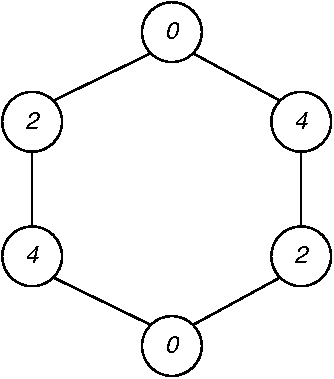
\includegraphics[width=0.522\linewidth]{circle_radiocolor.pdf}
      \caption{6-cycle graph radio coloring}
      \label{fig:circle_radiocolor}
   \end{subfigure}%
   \begin{subfigure}{.45\textwidth}
      \centering
      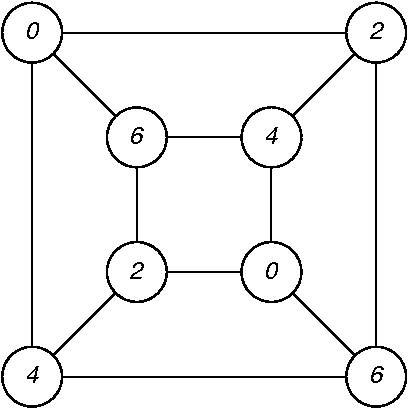
\includegraphics[width=0.6\linewidth]{cube_radiocolor.pdf}
      \caption{3-dimensional cube graph radio coloring}
      \label{fig:cube_radiocolor}
   \end{subfigure}
   \caption{Graph radiocoloring examples.}
   \label{fig:radiocolor_example}
\end{figure}

Although exact solutions for specific graphs such as paths, cycles, trees, cliques, and stars can be found, the problem remains NP-complete when restricted to planar, bipartite, chordal, and split graphs~\cite{yeh2006_dist2label_survey}\cite{deo2003_parallel_radiocoloring}.  Algorithms for finding exact solutions for \emph{k}-coloring are based on trying all $k^n$ assignments of \emph{k} colors to \emph{n} vertices and then checking the assignment validity. This can be achieved in $2^n n^{O(1)}$ time~\cite{bjorklund2009_setpart}. In order to minimize the required time or provide a solution to other types of graphs, various heuristic approaches exist. These typically work in $O(n^3)$ time. Nevertheless, heuristics do not aim to find an optimal solution (the least possible chromatic number) but rather find one of the possible solutions which may or may not be optimal. Therefore, various heuristics define upper and lower bounds on \emph{k}-chromatic number $r_{ck}$ they may find. The lower (closer to the optimal $r_{ck}$) the bounds are, the better a heuristic method is considered to be.

The following sections will compare two heuristic approaches based on~\cite{laxman2012_radio_k-coloring} and~\cite{deo2003_parallel_radiocoloring}. One of the approaches will be parallelized, and achieved experimental results will be discussed. Since the original proposal considered $L(2,1)$ labeling, we will implicitly consider $k=2$ for the rest of the paper. Nevertheless, the algorithm described in Section~\ref{sec:alg_sequential} provides computation for any $k$ by default. The algorithm in Section~\ref{sec:alg_parallel} can be easily modified to support any $k$ without changing its time or space complexity classes.

%%%%%%%%%%%%%%%%%%%%%%%%%%%%%%%%%%%%%%%%%%%%%%%%%%%%%%%%%%%%%%%%%%%%%%%%%%%%%%%%

\section{Sequential Algorithm}
\label{sec:alg_sequential}

In this section, we describe the sequential algorithm \textit{A~Graph Radio k-Coloring Algorithm} by Laxman Saha and Pratima Panigrahi~\cite{laxman2012_radio_k-coloring}. It works with undirected graphs in the representation of the adjacency matrix. It expects the graph to be connected. However, the algorithm can be easily modified to work with unconnected graphs as well. The procedure would be called for every unconnected part of the graph. The parameter $k$ can be specified as any natural number.

\subsection{Description}

The algorithm consists of three steps. Firstly, the shortest path between all pairs of vertices (the distance matrix) is computed. For this purpose, the procedure uses the Floyd-Warshall algorithm~\cite{wiki_floyd_warshall}.

\bigskip
\begin{lstlisting}
    distance_matrix = floyd_warshall(adjacency_matrix)
\end{lstlisting}
\bigskip

The second step is to compute the auxiliary matrix $c$. Its size is $n \times n$ ($n$ is the number of vertices), and every member is initialized to $\infty$. Then it is filled in the following way:

\bigskip
\begin{lstlisting}
    for i in (0 ... n):
        for j in (0 ... n):
            if k + 1 >= distance_matrix[i][j]:
                c[i][j] = k + 1 - distance_matrix[i][j]
            else:
                c[i][j] = 0
            c[j][i] = c[i][j]
        c[i][i] = INF
\end{lstlisting}
\bigskip

In the last step, we create an array $labels$ of size $n$ and initialize all its members to $\infty$. We choose any vertex (etc. $0$) and assign any label (etc. $0$) to it. Labels are represented by natural numbers. We also need another auxiliary variable $r$, which is the index of the last colored vertice ($0$ at the beginning). After the initialization, we perform the following loop.

\bigskip
\begin{lstlisting}
    repeat(n - 1):
        min_label = INF
        p = None
        for j in (0 ... n):
            if min_label > c[r][j]:
                min_label = c[r][j]
                p = j
        for j in (0 ... n):
            c[p][j] += min_label
        for j in (0 ... n):
            if c[p][j] < c[r][j]:
                c[p][j] = c[r][j]
        labels[p] = min_label
        r = p
\end{lstlisting}
\bigskip

After this step, the array $labels$ is filled, and so all of the vertices have their number assigned.

\subsection{Time complexity}

This subsection analyzes the time complexity of the algorithm as follows:

The time complexity of the first step -- Floyd-Warshall algorithm:

$$\textrm{DTIME} \approx O(n^2) + O(n^3) \approx O(n^3)$$

The time complexity of the second step -- initialization and filling the auxiliary matrix $c$:

$$\textrm{DTIME} \approx O(n^2) + O(n^2) \approx O(n^2)$$

The time complexity of the third step -- getting the labels $c$:

$$\textrm{DTIME} \approx O(n) \cdot ( O(n) + O(n) + O(n)) \approx O(n^2)$$

Thus the overall time complexity for the sequential algorithm:

$$\textrm{DTIME} \approx O(n^3) + O(n^2) + O(n^2) \approx O(n^3)$$

\subsection{Space complexity}

When analyzing the space complexity of the algorithm, we need to consider a space for the adjacency matrix of the input graph, the distance matrix computed by Floyd–Warshall algorithm, the auxiliary matrix $c$ for the main part, and the array for storing $labels$. Therefore, the overall space complexity for the sequential algorithm is

$$\textrm{DSPACE} \approx O(n^2) + O(n^2) + O(n^2) + O(n) \approx O(n^2)$$

%%%%%%%%%%%%%%%%%%%%%%%%%%%%%%%%%%%%%%%%%%%%%%%%%%%%%%%%%%%%%%%%%%%%%%%%%%%%%%%%

\section{Parallel Algorithm}
\label{sec:alg_parallel}

The implementation of the parallel algorithm was implemented according to N. Deo's paper \emph{Parallel Algorithm For Radiocoloring a Graph}~\cite{deo2003_parallel_radiocoloring}. The mentioned paper presents an approximation algorithm for a graph radio coloring with lower and upper bounds of the radiochromatic number $r_{ck}(G)$ derived from the Nordhaus-Gaddum theorem~\cite{nordhaus1956_compgraphs}. In this section, we will denote a radiochromatic number as $\lambda(G)$ as a special case of $r_{ck}(G)$ for $k=2$ to correspond with the original paper. Therefore, complementary graphs $G$ and $\overline{G}$, and their respective radiochromatic numbers $\lambda(G)$ and $\lambda(\overline{G})$ must satisfy the following conditions (Proof~\cite{deo2003_parallel_radiocoloring}):

$$ 2 \sqrt{2} \leq \lambda(G) + \lambda(\overline{G}) \leq 3n - 3$$
$$ 0 \leq \lambda(G) \cdot \lambda(\overline{G}) \leq \bigg(\frac{3n-3}{2}\bigg)^2$$

As mentioned in the previous section, the original algorithm considers only a radio coloring value of $k=2$ and is implemented in this manner. Nevertheless, it could be easily modified to support any $k$ with no change in the time complexity class. Although not explicitly stated in the paper, the authors have noticed that the used \emph{largest-degree first} heuristics resembles a search method for constraint satisfaction problems (CSP) min-conflict\footnote{\url{https://en.wikipedia.org/wiki/Min-conflicts_algorithm}} with the heuristics of most-constraining values first. For this reason, the algorithm has relatively low space requirements, which will be elaborated on later in this section.

\subsection{Description}
\label{ssec:parallel_description}

The algorithm expects input in the form of an adjacency matrix. Its initialization process is then split into three stages:

\begin{enumerate}
   \item Sort the vertices in descending order by their degree.
   \item Compute distance 2 binary matrix.
   \item Initialize a $n$ x $2n - 1$ \emph{"forbidden"} binary matrix signalizing whether a color identified by the column index can be used to color a vertex identified by the row index. If we consider a fully-connected graph, the maximum number of radio colors is $2n - 2$, hence the used matrix size.
\end{enumerate}

After the previous process is completed, the algorithm iterates over the list of sorted vertices and determines the next smallest color that can be given to the vertex. To determine the color $c$ for the vertex $v$, the forbidden matrix is consulted. When the next color $c$ is chosen, the forbidden matrix needs to be updated so that no conflict will occur in the next iteration. Therefore, we set the values of the columns corresponding to $c-1$, $c$, and $c+1$ in the forbidden matrix to 1 for all neighbors of $v$. Also, entries corresponding to $c$ need to be set for all nodes in the distance of $2$ from $v$. This way, the algorithm eventually assigns colors to all the vertices while respecting all radio coloring constraints.

\subsection{Parallelization}
\label{ssec:parallel_parallelization}

The paper suggests that the initialization phase can be fully parallelized. Therefore, we parallelized sorting by a custom implementation of a parallel merge sort as suggested by~\cite{bukata_advancedOpenMP}. The distance 2 matrix computation could be parallelized by letting each processor compute each matrix row independently. Initialization of matrix "forbidden" to 0s was straightly done in the serial environment via the object constructor, thus no parallel initialization was needed. The process of coloring was also parallelized, such that accessing the matrix "forbidden", both for searching for the smallest color and updating the matrix after the color assignment is done by multiple processors.

The author of the original paper suggests that the implementation should use $n$ processors (equal to the number of graph vertices) for the maximum performance. Since this is unrealistic in our scenario, we implemented the solution in C++ and parallelized it with OpenMP\footnote{API specification for parallel programming. See \url{https://www.openmp.org/}}. OpenMP supports native load-balancing of work according to the number of available threads. Therefore, our solution is both scalable and robust as it can distribute the work for any number of available processors. This fact implies that the implementation can also work with only one thread, thus in a fully serial mode without additional changes to the code.

For the purpose of comparing sequential and parallel implementations, the parallel variant should use all the available threads. However, spawning the threads and their termination may add significant overhead, causing the parallelized solution to be inefficient. For this reason, we added a compilation macro \texttt{PARALLEL\_OPTIMIZED}, which causes the algorithm to execute itself sequentially if the parallel version would be inefficient. For example, instead of parallel recursive execution of MergeSort, we simply call C++ standard library sequential function \texttt{sort()} for small-sized lists, which execution is much more efficient. Comparison of full parallelized mode and our optimized variant will be further discussed in Section~\ref{sec:eval}.

\subsection{Time Complexity}
\label{ssec:parallel_timeComplex}

To analyze the algorithm's complexity, we will first look at its sequential variant: The vertex's degree is computed by counting the number of 1s in each adjacency matrix row -- $O(n^2)$. Used sorting algorithm (MergeSort) is optimal, hence $O(n \log n)$. Computation of distance 2 matrix requires checking all neighbors for each element in each row -- $O(n^3)$. The final step needs to assign a color for each vertex. In each of these assignments, we first have to choose the color by iterating through the row of the given vertex in the forbidden matrix and then update the forbidden matrix for all neighbors after the color has been assigned -- $O(n^3)$. Therefore, we calculate the algorithm time complexity as:

$$\textrm{DTIME} \approx O(n^2) + O(n \log n) + O(n^3) + O(n^3) \approx O(n^3)$$

When we consider a parallel environment with $n$ processors and take into account that each of the algorithm parts can be parallelized as described above, the time complexity would be:

$$\textrm{DTIME}_n \approx O(n) + O(\log n) + O(n^2) + O(n \log n) \approx O(n^2)$$

Note that the color assignment process has improved from $O(n^3)$ to $O(n \log n)$ due to the ability to perform parallel reduction on a tree in $O(\log n)$ time to find the minimum available color. Our implementation also performs a variant of a local reduction in $O(N/P)$, where $P$ is the number of processors and then an OpenMP \texttt{min} reduction in order to find the minimum in $O(log n)$ time. Performing the operation for each vertex cannot be parallelized, thus we obtain $O(n \log n)$ time. Multiplying the overall complexity $O(n^2)$ by the theoretical number of processors gives us $O(n^3)$, which is the same as the sequential variant. The parallel algorithm is thus optimal. Since we are not using exactly $n$ processors in our experiments, note that the actual complexity would be calculated by dividing sequential variant by the number of processors. Therefore, we would get $\approx O\Big(\frac{n^3}{P}\Big)$, where $P$ is the number of processors. However, the resulting algorithm would still be optimal.

\subsection{Space Complexity}
\label{ssec:parallel_spaceComplex}

Since the algorithm is a heuristics, it does not need to remember any intermediate calculations. The space complexity is thus negligible from the practical point of view. From the theoretical perspective, the space complexity computation must consider three vectors containing vertex degrees, sorted vertices, and colorings, all of $O(n)$. Also, the input matrix and the distance 2 matrix with $O(n^2)$ as well as the forbidden matrix, sized $n$ x $2n -1$ as $\sim O(2n^2)$. Therefore, we define space complexity as:

$$\textrm{DSPACE} \approx O(n) + O(n) + O(n) + O(n^2) + O(n^2) + O(2 n^2) \approx O(n^2)$$

%%%%%%%%%%%%%%%%%%%%%%%%%%%%%%%%%%%%%%%%%%%%%%%%%%%%%%%%%%%%%%%%%%%%%%%%%%%%%%%%

\section{Program Usage}
\label{sec:prog_usage}

The algorithms described in previous sections are implemented as a part of a standalone C++ program \texttt{gal} located in the \texttt{src/} directory. Compilation of the program is done with \texttt{make}. The user may alternatively use \texttt{make paropt} to compile an optimized parallel version of the algorithm described in Section~\ref{sec:alg_parallel}. The program is then run by specifying the algorithm to be run using \texttt{-s} for sequential (implicit) or \texttt{-p} for parallel version. The parallel version may be specified the number of threads to use a with the option \texttt{-t NUM}. If the time is desired to be measured, the option \texttt{-m} should be used. Finally, an input graph in the form of the file has to be specified as the last non-option program argument. The graph structure requires an adjacency matrix specification in a strict 1-line JSON format (printed python array). For example, the following file specifies an adjacency matrix for a graph with three vertices:

\noindent \texttt{[[0,1,1],[1,0,1],[1,1,0]]\textbackslash n} \\
\texttt{EOF}
\vspace{0.5em}

The specification of the $n$\,x\,$n$ adjacency matrix follows the graph theory conventions -- connections for each node are represented with a row $i$, where column $j$ contains a value of 0 or 1. 1 defines an~existing connection between the nodes with indices $i$ and $j$, whereas 0 defines a non-existing connection between these nodes.

After the program is run, it prints the result of the chosen coloring algorithm as a series of integers delimited by a space. Each value represents a color assigned to the vertice on the particular index. For example, output \texttt{4 2 0} represents a valid coloring given to the fully-connected graph with three vertices, as given in the example before. In this coloring, we assign color $4$ to the node with index \emph{0}, color $2$ to the node with index \emph{1}, and finally, color $0$ to the node with index \emph{2}. If the time measurement (option \texttt{-m}) is specified, its result in milliseconds is printed on the second line. Please refer to the \texttt{-h}/\texttt{--help} option for further information about the program usage.

The process of data generation, time measurements, and results evaluation is automatized with scripts \texttt{generate\_graphs.py}, \texttt{get\_plots.py}, and \texttt{run\_measurements.py} placed in the \texttt{scripts/} directory. Firstly, the script \texttt{generate\_graphs.py} is used to create a predefined number of connected graphs with the given number of nodes. For the demonstration's ease and speed, we use graphs from 5 up to 200 nodes with the step 5, whereas the script creates 10 of each and saves them in the \texttt{data\_graphs/} folder. These settings can be controlled at the top of the script by updating the appropriate variable.

After the graphs are generated, script \texttt{run\_measurements.py} is used to run the program for all the data in \texttt{data\_graphs/} directory. Variable \texttt{VARIANTS} defines which version of the algorithm should be run, \texttt{s} meaning serial version, and \texttt{pX} meaning parallel version with X threads. For this reason, more of the program variants can be run with a single script run. All the measured results are saved in the \texttt{data\_times/} directory.

Finally, the measured results can be aggregated and visualized using script \texttt{get\_plots.py}, which takes data from \texttt{data\_times/} and generates plots into the \texttt{plots/} directory in \textit{png} format for each algorithm variant. Axis "y" in the graphs denotes the median of all the measured times in milliseconds for a particular algorithm variant with respect to the size of the graph. Axis "x" denotes the number of vertices of the graph. Custom graph titles (or specifications for other parallel program runs) can be made by changing the \texttt{get\_title} dictionary variable at the top of the file.

Note that all three scripts require that their particular output directory (\texttt{data\_graphs/}, \texttt{data\_times/}, and \texttt{plots/}) does not exist when the scripts are run. If the directory exists, the script will fail. This feature is implemented to prevent accidental overwriting of the existing results by another script run.

To offer all of the previously described functionality in a single-run solution, the script \texttt{run.sh} is also provided. The script automatically compiles the program binaries and runs all three previously described scripts with their defined settings.

%%%%%%%%%%%%%%%%%%%%%%%%%%%%%%%%%%%%%%%%%%%%%%%%%%%%%%%%%%%%%%%%%%%%%%%%%%%%%%%%

\section{Evaluation}
\label{sec:eval}

Evaluation of the described algorithms was performed on 15.12.2020 and 16.12.2020 on the faculty server \texttt{merlin.fit.vutbr.cz} by running them on input graphs with various sizes for up to 1000 nodes. Each graph size contained between 20 and 50 graphs (according to their size), algorithms computed results for each graph, and the median was used to represent the final result. The data were generated by the \texttt{generate\_graphs.py} script and run with \texttt{run\_measurements.py} during the night to minimize server load, which may skew the results due to thread context switches. The machine running merlin contains a processor Intel(R) Xeon(R) CPU E5-2640 0 @ 2.50GHz with 12 physical CPUs and two threads per core. For this reason, we will use up to 16 threads during our tests since using significantly more threads than available physical cores tend to degrade the performance instead of improving it.

\subsection{Sequential Algorithms Comparison}
\label{ssec:seq_comps}

\begin{figure}[t]
   \centering
   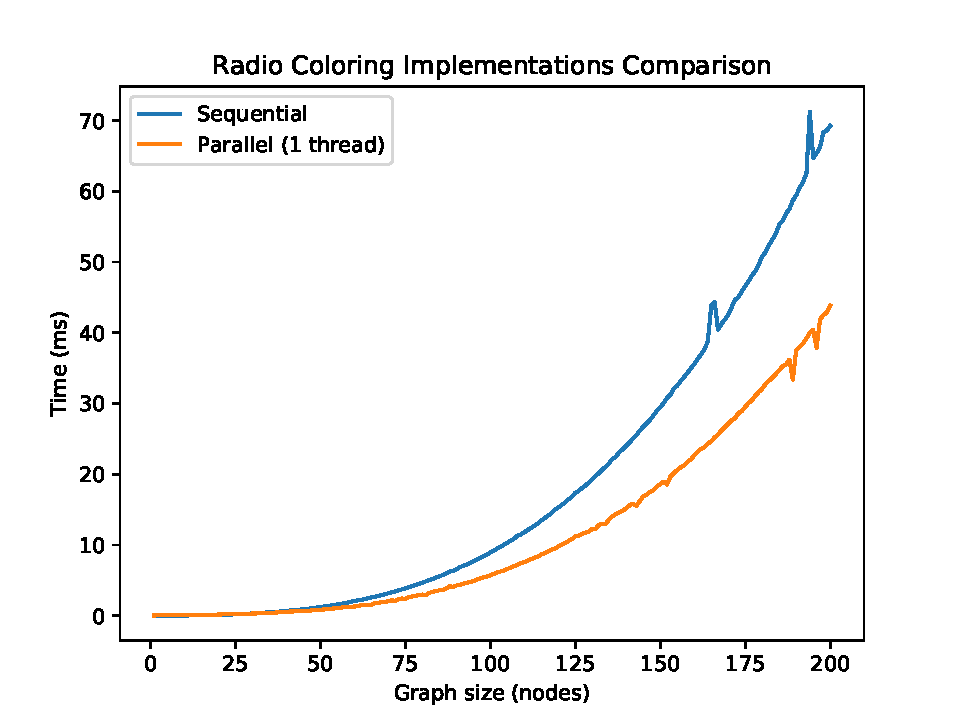
\includegraphics[width=0.6\linewidth]{seq_impl_comparison.pdf}
   \caption{Graph radiocoloring sequential implementations comparison.}
   \label{fig:seq_impl_comparison}
\end{figure}

Since the parallel implementation is not necessarily bound to the parallel environment, we decided to compare the performances of pure sequential and parallel variant with one thread as our very first test (Figure~\ref{fig:seq_impl_comparison}). For this purpose, we used smaller graphs with up to 200 nodes and option \texttt{-t 1} to specify only 1 thread run. As it may be seen from the figure, both curves are beginning to resemble quadratic, nearly cubic behavior, as would correspond to time complexity $O(n^3)$ of both implementations. The cubic behavior would surely be shown better for graphs with a bigger number of vertices. Nevertheless, despite both implementations having the same complexity class, the second implementation supporting parallel execution performs much better in general. On the other hand, the quality of the heuristics for the pure sequential algorithm has been empirically shown to be slightly better, often finding a~lower radiochromatic number than the parallelized variant. Because there is such a difference between implementations, we will be mentioning them together in future comparisons for better illustration.

\subsection{Pure Parallel And Optimized Parallel Comparison}
\label{ssec:par_paropt}

As mentioned in Sections~\ref{sec:alg_parallel} and~\ref{sec:prog_usage}, the parallel version also supports an optimized variant that does not perform parallel computations if not necessary, thus saving system resources for thread management. Figure~\ref{fig:paropt_comparison} beautifully shows this property for smaller graphs processed by 16 threads. As it may be seen, there are two jumps at $n=32$ and $n=64$ for an optimized parallel variant. These are the places when parallelized computation got into effect. Due to the poor choice of graph size, the parallelization got into effect a bit sooner than desired, hence still creating unwanted thread management overhead such as in a pure parallel graph. On the other hand, the optimized variant was slightly more efficient in values under 64 due to this fact. After the parallelization was fully active, the graphs resembled roughly the same shape. Note that adjusting the values to switch parallelism a bit later on may further increase the computation performance. As one may think at this point -- "Why do we even parallelize when the sequential version is better anyway?". This is, indeed, not true. An example with 16 threads was chosen to better illustrate optimized algorithm functionality, but 16 threads are more than available 12 physical processors,  and so frequent context switching causes performance degradation. In contrast, Figure~\ref{fig:par_paropt8} compares the parallel version with 1 thread to the optimized parallel version with 8 threads. As evident from the figure, the sequential version was outperformed in graph sizes somewhere between 60-70 elements, and the performance of the parallel version with 8 threads was significantly better later on. Also, note that the parallel version with 8 threads performed much better than its counterpart with 16 threads due to the problems described above.

\begin{figure}[t]
   \centering
   \begin{subfigure}{.45\textwidth}
      \centering
      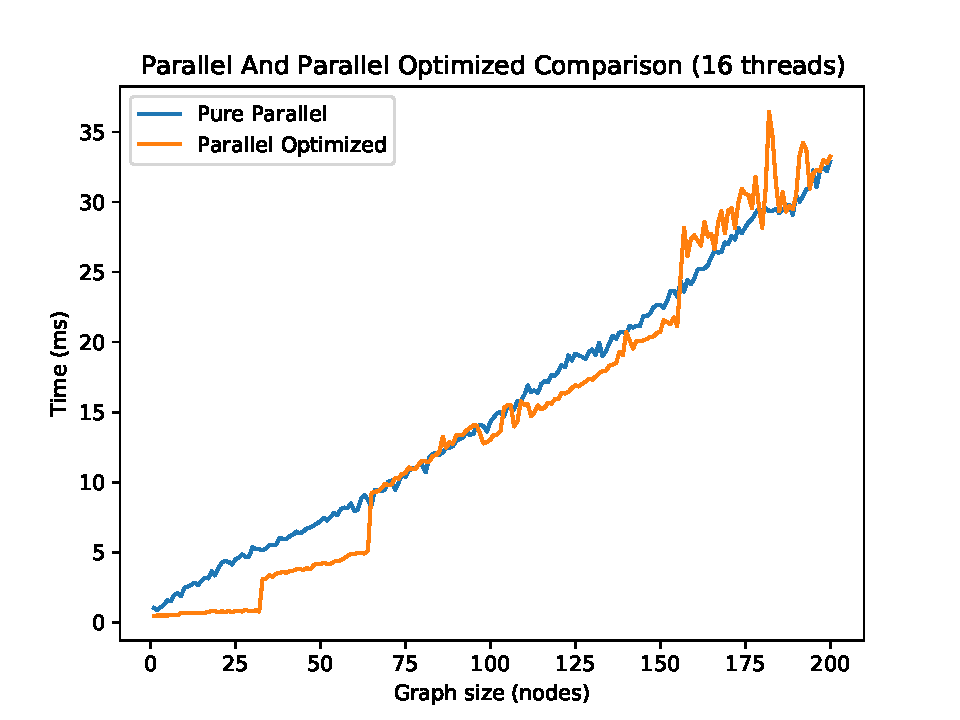
\includegraphics[width=\linewidth]{par_paropt16.pdf}
      \caption{Pure parallel vs. optimized parallel \\comparison for 16 threads.}
      \label{fig:paropt_comparison}
   \end{subfigure}%
   \begin{subfigure}{.45\textwidth}
      \centering
      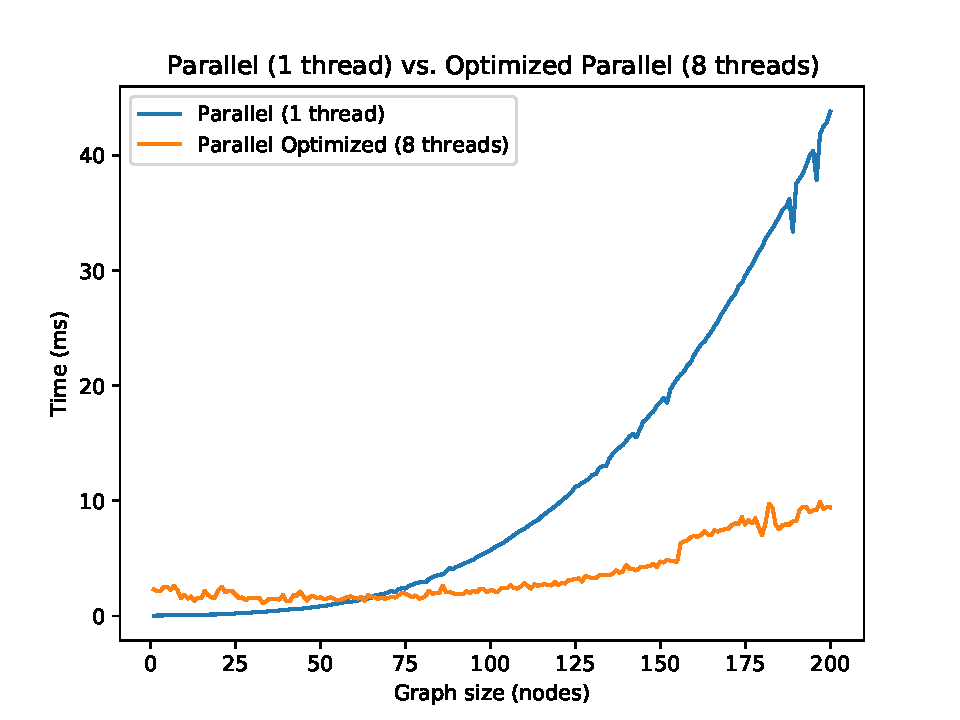
\includegraphics[width=\linewidth]{par1_optPar8.pdf}
      \caption{Optimized parallel (8 threads) vs. \\parallel (1 thread)}
      \label{fig:par_paropt8}
   \end{subfigure}
   \caption{Optimized Parallel Algorithm Functionality}
   \label{fig:paropt}
\end{figure}

\subsection{Comprehensive Algorithms Comparison}
\label{ssec:comp_comprehensive}

For the sake of completeness, we also present algorithm runs for the bigger graphs up to $1000$ nodes. These will be presented mostly without commentary since algorithm functionality, and general trends of their scaling could have been picked up from the previous subsections. The first graph compares 1-threaded implementations, and each other graph describes the performance improvement due to multiprocessing compared to both 1-threaded variants.

\begin{figure}[H]
   \centering
   \begin{minipage}{.45\textwidth}
      \centering
      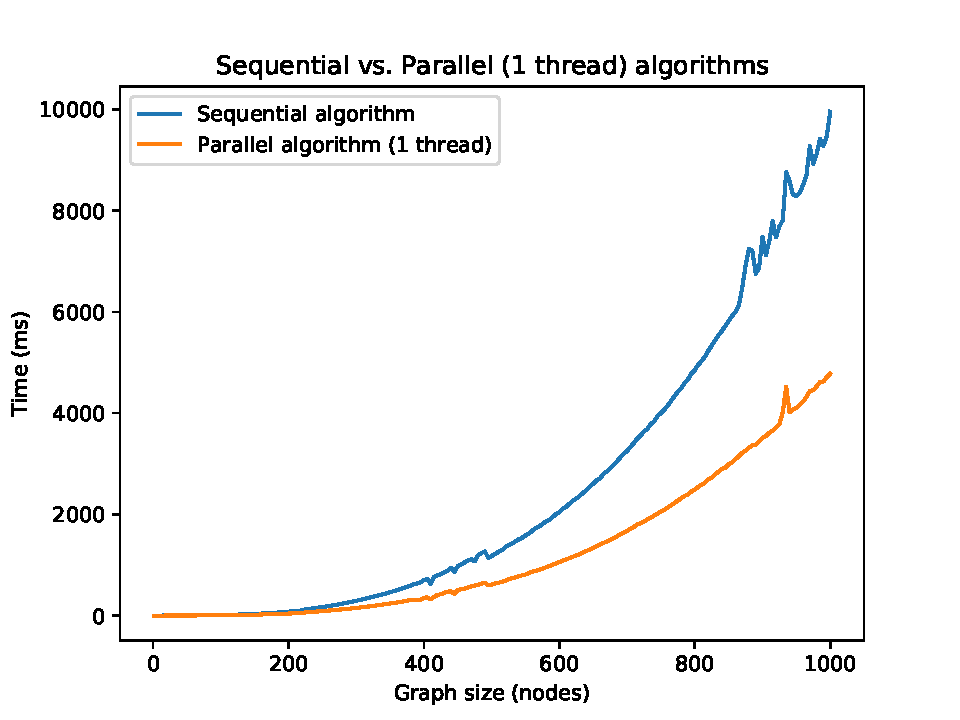
\includegraphics[width=\linewidth]{comp_1thread.pdf}
      \caption{1-thread implementations\\comparisons.}
      \label{fig:comp_1thread}
    \end{minipage}%
   \begin{minipage}{.45\textwidth}
      \centering
      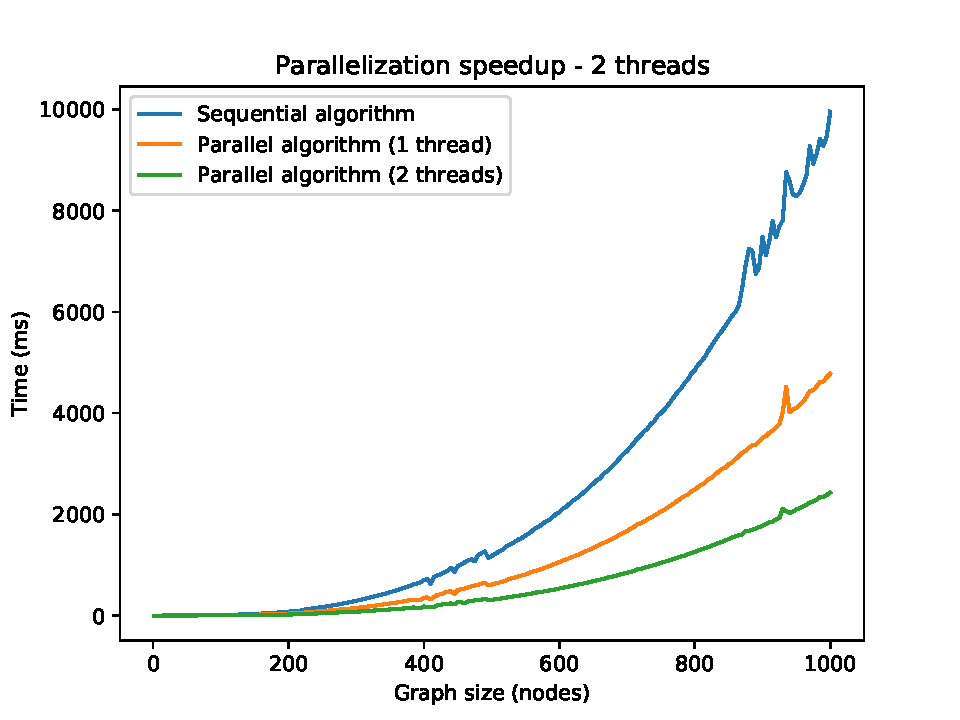
\includegraphics[width=\linewidth]{comp_2thread.pdf}
      \caption{2-threads parallelization speed-up.}
      \label{fig:comp_2thread}
   \end{minipage}%
   \label{fig:comprehensive_comp1}
\end{figure}
\vspace{-1.5em}
\begin{figure}[H]
   \centering
   \begin{minipage}{.45\textwidth}
      \centering
      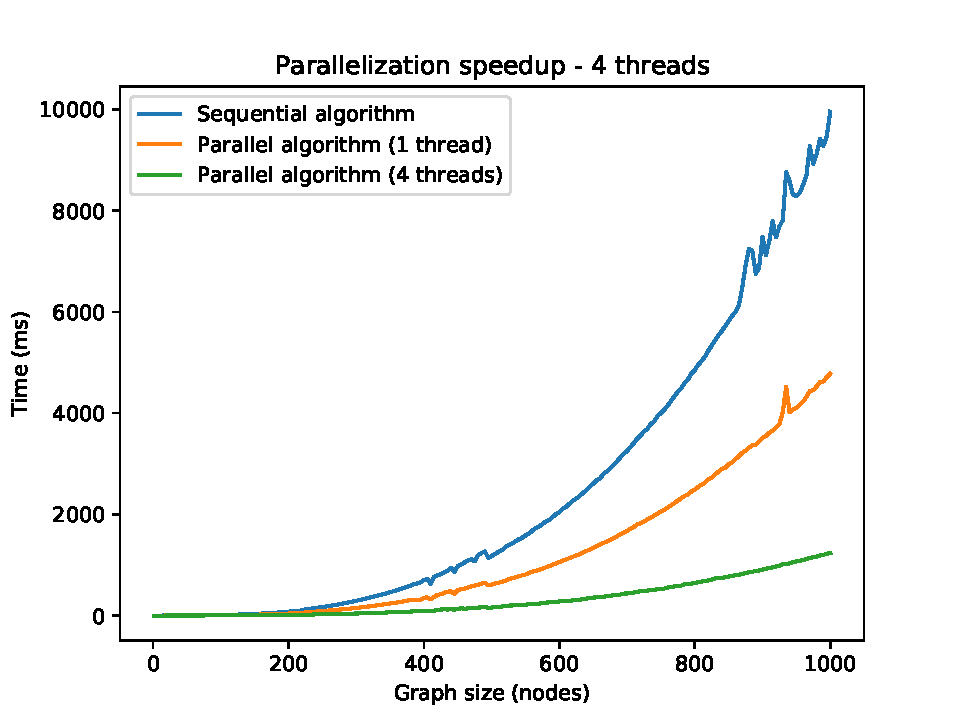
\includegraphics[width=\linewidth]{comp_4thread.pdf}
      \caption{4-threads parallelization speed-up.}
      \label{fig:comp_4thread}
   \end{minipage}%
   \begin{minipage}{.45\textwidth}
      \centering
      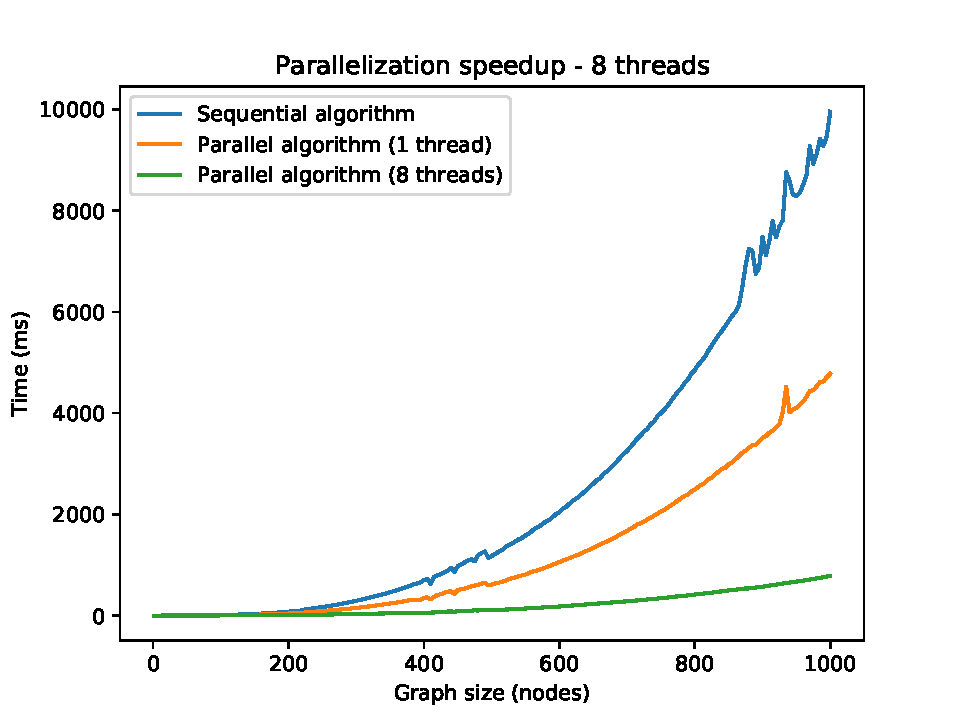
\includegraphics[width=\linewidth]{comp_8thread.pdf}
      \caption{8-threads parallelization speed-up.}
      \label{fig:comp_8thread}
   \end{minipage}%
   \label{fig:comprehensive_comp2}
\end{figure}
\vspace{-1.5em}
\begin{figure}[H]
   \centering
   \begin{minipage}{.5\textwidth}
      \centering
      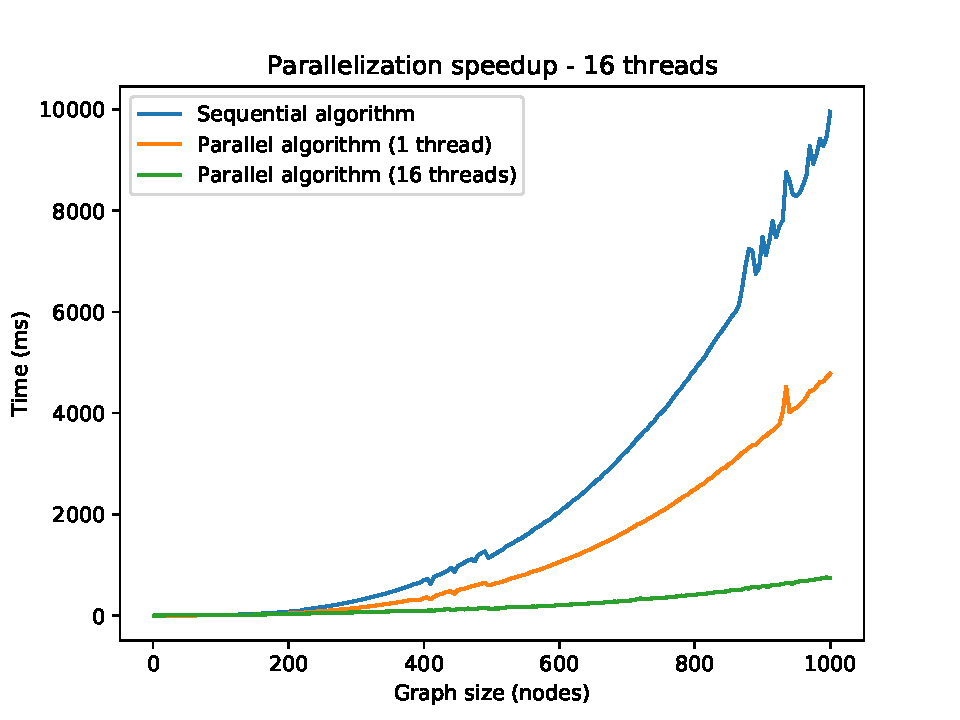
\includegraphics[width=0.9\linewidth]{comp_16thread.pdf}
      \caption{16-threads parallelization speed-up.}
      \label{fig:comp_16thread}
   \end{minipage}%
\end{figure}

%%%%%%%%%%%%%%%%%%%%%%%%%%%%%%%%%%%%%%%%%%%%%%%%%%%%%%%%%%%%%%%%%%%%%%%%%%%%%%%%

\section{Conclusions}
\label{sec:conclusions}

This paper has discussed the problem of radio coloring a graph, provided its definition, described and implemented two approximate algorithms to solve it, and performed various tests in a parallelized environment to verify the time complexity of the algorithms. As may be seen from Figures~\ref{fig:comp_2thread}-\ref{fig:comp_16thread}, using more threads always significantly improved the time needed to color the graph. The achieved performance was best with 8 and 16 threads. Their curve is almost the same because machine \texttt{merlin.fit.vutbr.cz} on which the tests were performed provides only 12 physical cores, thus using more threads than this number is inefficient and brings no befit. Two processors provided a speed-up of 1.966 when compared to its 1-threaded algorithm variant and speed-up of 4.096 with respect to the pure sequential algorithm. Speed-ups are increasing as more processors are added in an "almost" linear fashion up to the eight processors. By implementing and measuring algorithms' performance in practice, we conclude that the problem of radio coloring can be efficiently solved in the parallel environment and the achieved speed-up closely corresponds to the theoretical expectations up to the limits of the hardware.

%%%%%%%%%%%%%%%%%%%%%%%%%%%%%%%%%%%%%%%%%%%%%%%%%%%%%%%%%%%%%%%%%%%%%%%%%%%%%%%%

\begin{thebibliography}{1}
   \bibitem{laxman2012_radio_k-coloring} LAXMAN Saha and PRATIMA Panigrahi. \textit{A~Graph Radio k-Coloring Algorithm}. July 2012. In \emph{International Workshop on Combinatorial Algorithms}. DOI: 10.1007/978-3-642-35926-2\_15.

   \bibitem{deo2003_parallel_radiocoloring} DEO N. and BALAKRISHNAN H. \textit{ParallelL Algorithm For Radiocoloring a Graph}. January 2003.

   \bibitem{wiki_graphcoloring} Wikipedia contributors \textit{Graph coloring --- {Wikipedia}{,} The Free Encyclopedia}. 2020. [Online; accessed 15-December-2020]. Available at: \url{https://en.wikipedia.org/wiki/Graph_coloring}.

   \bibitem{marx2003_graphcolouring} \emph{Graph Colouring Problems And Their Applications in Scheduling}. December 2003. In \emph{Periodica Polytechnica, Electrical Engineering, Vol. 48}.

   \bibitem{chaitin1982_regalloc} CHAITIN G. J. \emph{Register Allocation \& Spilling Via Graph Coloring}. June 1982. In \emph{SIGPLAN Symposium on Compiler Construction, Vol. 17}.

   \bibitem{rosenhouse2012_sudoku} ROSENHOUSE Jason and TAALMAN Laura. \emph{Taking Sudoku Seriously: The Math Behind the World's Most Popular Pencil Puzzle}. 2011. Oxford University Press, Inc. ISBN 978-0-19975656-8.

   \bibitem{badr_exact_parallel_radiocolor} BADR El-Sayed and ALOUFI Khalid. \emph{An Exact Parallel Algorithm for the Radio k-coloring Problem}. November 2019. In \emph{Preprints 2019}. DOI: 10.20944/preprints201911.0232.v1.

   \bibitem{griggs1992_21_labeling} GRIGGS R. Jerold and YEH K. Roger. \emph{Labelling Graphs with a Condition at Distance 2}. November 1992. In \emph{SIAM Journal on Discrete Mathematics, Vol. 5}.

   \bibitem{yeh2006_dist2label_survey} YEH K. Roger. \emph{A~Survey on Labeling Graphs With a Condition at Distance Two}. June 2006. In \emph{Discrete Mathematics, Vol. 306}.

   \bibitem{bjorklund2009_setpart} BJ\"{O}RKLUND Andreas, HUSFELDT Thore, KOIVISTO Mikko. \emph{Set Partitioning via Inclusion-Exclusion}. June 2009. In \emph{SIAM Journal on Computing, Vol. 39}. Published by Society for Industrial and Applied Mathematics. DOI: 10.1137/070683933.

   \bibitem{wiki_floyd_warshall} Wikipedia contributors \textit{Floyd–Warshall algorithm --- {Wikipedia}{,} The Free Encyclopedia}. 2020. [Online; accessed 16-December-2020]. Available at:
      \url{https://en.wikipedia.org/wiki/Floyd-Warshall\_algorithm}.

   \bibitem{nordhaus1956_compgraphs} NORDHAUS E. A. and J. W. GADDUM. \emph{On Complementary Graphs}. The American Mathematical Monthly. Mathematical Association of America, 1956, 63(3), 175-177. ISSN 00029890.

   \bibitem{bukata_advancedOpenMP} BUKATA Libor and DVO\v{R}\'{A}K JAN. \emph{Advanced Programming With OpenMP}. Faculty of Electrical Engineering, Czech Technical University in Prague. 2018. [Online; accessed 16-December-2020]. Available at: \url{https://cw.fel.cvut.cz/old/_media/courses/b4m35pag/lab6_slides_advanced_openmp.pdf}

\end{thebibliography}

%%%%%%%%%%%%%%%%%%%%%%%%%%%%%%%%%%%%%%%%%%%%%%%%%%%%%%%%%%%%%%%%%%%%%%%%%%%%%%%%

\end{document}
